\documentclass[14pt,a4paper,onecolumn]{extarticle}
\usepackage[utf8]{inputenc}
\usepackage{amsmath}
\usepackage{amsfonts}
\usepackage{amssymb}
\usepackage{graphicx}
\usepackage{natbib}
\usepackage{multirow}
\usepackage{pdflscape}

\bibliographystyle{plainnat}
\setlength{\parskip}{1.2em}
\setlength{\parindent}{0pt}
% \graphicspath{{./images/}}

\author{Ibrahim AbuBakr ElSeddiq}
\title{The predictive value of NTproBNP on postoperative outcome in patients undergoing offpump CABG}

\begin{document}

\maketitle
\clearpage

\tableofcontents
\clearpage

\listoffigures
\clearpage

\listoftables
\clearpage

\section{Introduction}

Coronary heart disease is the main cause of morbidity and mortality in developed countries, and the prevalence is increasing in developing countries.  Several studies have reported biomarker clusters which are associated with CHD.  The assessment of these biomarkers, alone or in combination, may improve the long-term prediction of mortality of first major cardiovascular event compared to conventional risk markers. \citep{Zethelius2008}

Brain type natriuretic peptide (BNP) is primarily produced by cardiac myocytes. Physiological effects of BNP are a peripheral vasodilatation and inhibition of renin-angiotensin production. \citep{DanielsandMaisel2007} The precursor peptide proBNP is split into the active hormone BNP and the N-terminal fragment (NT-proBNP).  Both BNP and NT-proBNP are established markers for cardiac failure.  NT-proBNP is also more stable, which makes its measurement more reliable. \citep{Thay-Hsiung2013} NT-proBNP was identified as a novel and important CHD biomarker, and has prognostic value in patients with stable CHD. \citep{Kragelund2005} A report from the BELSTRESS study suggested that NT-proBNP levels were a strong predictor of coronary events, even after adjustment for conventional risk factors. \citep{DeSutter2005} In patients with coronary artery disease increased BNP levels are associated with an increased  rate of myocardial infarction and cardiovascular death during mid-term follow-up. \citep{Schnabel2006}

However, Other pathologies such as exacerbated chronic obstructive pulmonary disease, atrial fibrillation, and myocarditis can cause elevated BNP levels. Additionally, higher NT-proBNP levels are associated with : female gender, impaired renal fuction, and older age.  Increased BNP levels are a prognostic marker associated with higher mortality in patients with myocardial infarction, cardiogenic shock, and pulmonary embolism. \citep{Rodseth2009}

\clearpage
\section{Review of Literature}

\subsection{Natriuretic Peptides}


In 1956, Kisch found that guinea pig atrial, but not ventricular, cells contained highly developed Golgi networks, similar to those observed in secretory cells \citep{Kisch1956}. Jamieson and Palade reported that atrial, but not ventricular, myocytes contain spherical, electron opaque granules \citep{Jamieson1964}. At the same time, physiological experiments conducted by Henry and colleagues revealed that balloon distension of the atria correlated with increased urination in dogs \citep{Henry1956}.

In a study published in 1981, de Bold and colleagues elegantly linked the seemingly disparate studies of Kisch and Henry by showing that atrial, but not ventricular, extracts contain a potent blood pressure decreasing component that works by stimulating renal sodium and water secretion \citep{deBold1981}. Shortly after the publication of this landmark paper, a number of groups reported the purification and sequencing of atrial peptides of varying sizes that possessed natriuretic, diuretic, and/or smooth muscle relaxing activity \citep{Currie1984}  \citep{Flynn1983} \citep{Kangawa1984} \citep{Misono1984}. Thus, the first natriuretic peptide was discovered.

 Several different names were given to these peptides such as atrial natriuretic factor, atriopeptin, cardionatrin, and cardiodilatin. However, atrial natriuretic peptide (ANP) is most often used to describe this peptide in the current literature. The second member of the family to be discovered, B-type natriuretic peptide (BNP), was originally called brain natriuretic peptide because it was purified and sequenced from porcine brain \citep{Sudoh1988}. However, subsequent studies found that it is more highly concentrated in cardiac ventricles of patients with heart failure \citep{Mukoyama1991}  \citep{Mukoyama1990}. Therefore, it is often described as B-type natriuretic peptide today. Finally, the third member of the family, C-type natriuretic peptide (CNP) was purified in 1991 from porcine brain extracts based on its ability to relax smooth muscle. All three members are similar in primary amino acid structure, contain a 17-residue disulfide ring, and are the products of separate genes.\citep{Sudoh1990}

 The biological actions of natriuretic peptides are mediated through membrane-bound natriuretic peptide receptors (NPR) that are linked to a cyclic guanosine monophosphate-dependent signaling cascade, including NPR-A, which preferentially binds ANP and BNP, and NPR-B, which preferentially binds CNP.

Elevated natriuretic peptides levels can be also found in many circumstances involving LV dysfunction or hypertrophy; right ventricular (RV) dysfunction secondary to pulmonary diseases; cardiac inflammatory or infectious diseases; and endocrinologic diseases and high output status without decreased left ventricular ejection fraction (EF), e.g., sepsis, renal failure, cirrhosis of liver, or intracranial pathologies. The causes and mechanisms of elevated natiuretic peptides levels are summarized in Fig. \ref{NP_causes}. The potential clinical applications in the non-HF settings are summarized in Table \ref{NP_applications}.

\begin{figure}
    \centering
    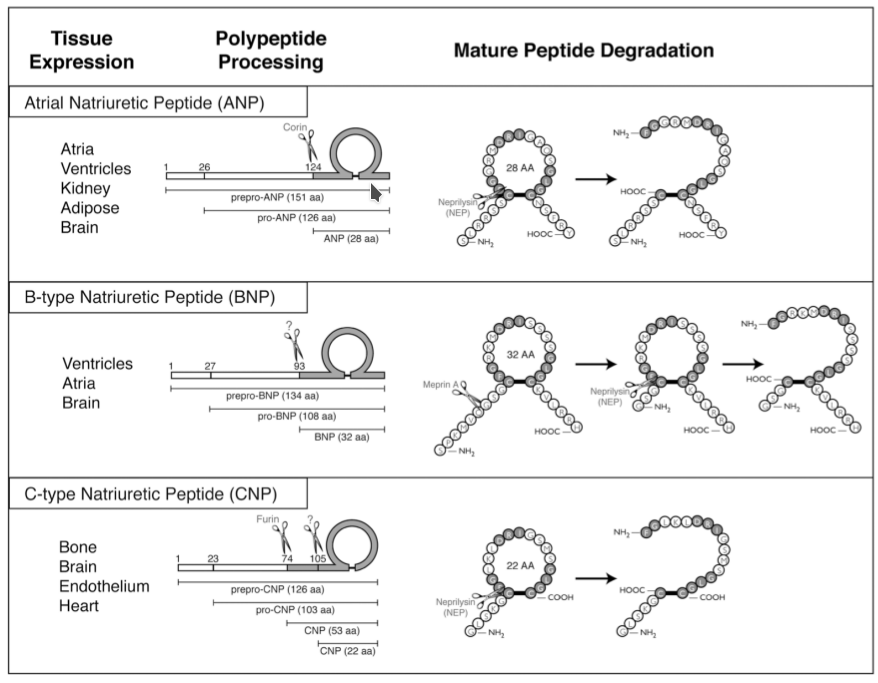
\includegraphics[scale=0.4]{./images/NP_structure.png}
    \caption{Structure of the human natriuretic peptides. The structure of the preprohormones for ANP, BNP and CNP are outlined on the left of each panel. The final amino acid sequence and structure of the mature peptides along with the major degradation product are shown on the right. The sites of cleavage are indicated with scissors.}
    \label{NP_structure}
\end{figure}

\subsubsection{Atrial Natriuretic Peptide}

All natriuretic peptides are synthesized as preprohormones Fig \ref{NP_structure}.
The resulting mRNA gives rise to a 151 amino acid polypeptide, known as preproANP. The first 25 amino acids constitute a signal sequence that is cleaved to yield a 126 amino acid peptide called proANP, which is the major form of ANP stored in the atrial granules \citep{Oikawa1984}.
Upon release from these granules, proANP is rapidly cleaved by corin, a transmembrane cardiac serine protease. Corin is highly expressed on the extracellular surface of atrial cardiomyocytes and cleaves proANP into the biologically active 28-amino acid form of ANP \citep{Yan2000}.
%Mice lacking functional corin have dramatically reduced levels of fully processed ANP in their hearts and are mildly hypertensive \citep{Chan2005}.
Alternative processing of proANP in the kidney by an unknown protease results in a 32-amino acid peptide called urodilatin that contains four additional amino-terminal residues \citep{Forssmann1998}.
Disruption of the murine ANP gene, results in marked hypertension, which was initially described as salt-sensitive \citep{John1995}, but later found not to be correlated with dietary salt intake \citep{John1996}.

Release of proANP from the atrial granules is primarily stimulated by stretch of the atrial wall caused by increased intravascular volume \citep{Bilder1986} \citep{Edwards1988} \citep{Lang1985}, but pressor hormones also stimulate ANP release \citep{Ruskoaho2003}.
%Upon secretion and cleavage into the mature peptide, ANP enters the coronary sinus and is distributed to its target organs via the circulation.
Plasma levels of ANP are relatively low (10 fmol/ml), but in patients with congestive heart failure, circulating ANP levels are elevated from 10- to 30-fold \citep{Burnett1986} \citep{Cody1986}.

The plasma half-life of ANP in humans is approximately 2 min \citep{Nakao1986} \citep{Yandle1986}.
Degradation of the active ANP peptide occurs through the actions of neutral endopeptidase (NEP) \citep{Stephenson1987} \citep{Vanneste1988} as well as through binding to the natriuretic peptide clearance receptor (NPR-C), a cell surface receptor that lacks guanylyl cyclase activity and controls the local concentrations of natriuretic peptides via constitutive receptor mediated internalization and degradation. Inhibiting NEP, increases the half-life of ANP \citep{Yandle1989},
suggesting that NEP activity contributes to the rapid clearance of ANP. However, it is important to note that mice lacking functional NEP do not exhibit increased natriuretic peptide function \citep{Lu1995}.
In contrast, mice lacking NPR-C are hypotensive, exhibit skeletal overgrowth and have reduced ability to clear ANP compared to wild type mice, suggesting that NPR-C is also a physiologic regulator of circulating natriuretic peptide concentrations \citep{Matsukawa1999}.

ANP is secreted in response to:
    \begin{itemize}
        \item Stretching of the atrial wall \citep{Widmaier2008}
        \item Reduced Sympathetic stimulation of $\beta$-adrenoceptors
        \item Raised sodium concentration (hypernatremia), though sodium concentration is not the direct stimulus for increased ANP secretion. \citep{Widmaier2008}
        \item Endothelin, a potent vasoconstrictor
        \item exercise \citep{Kokkonen2002}
    \end{itemize}


\begin{figure}
    \centering
    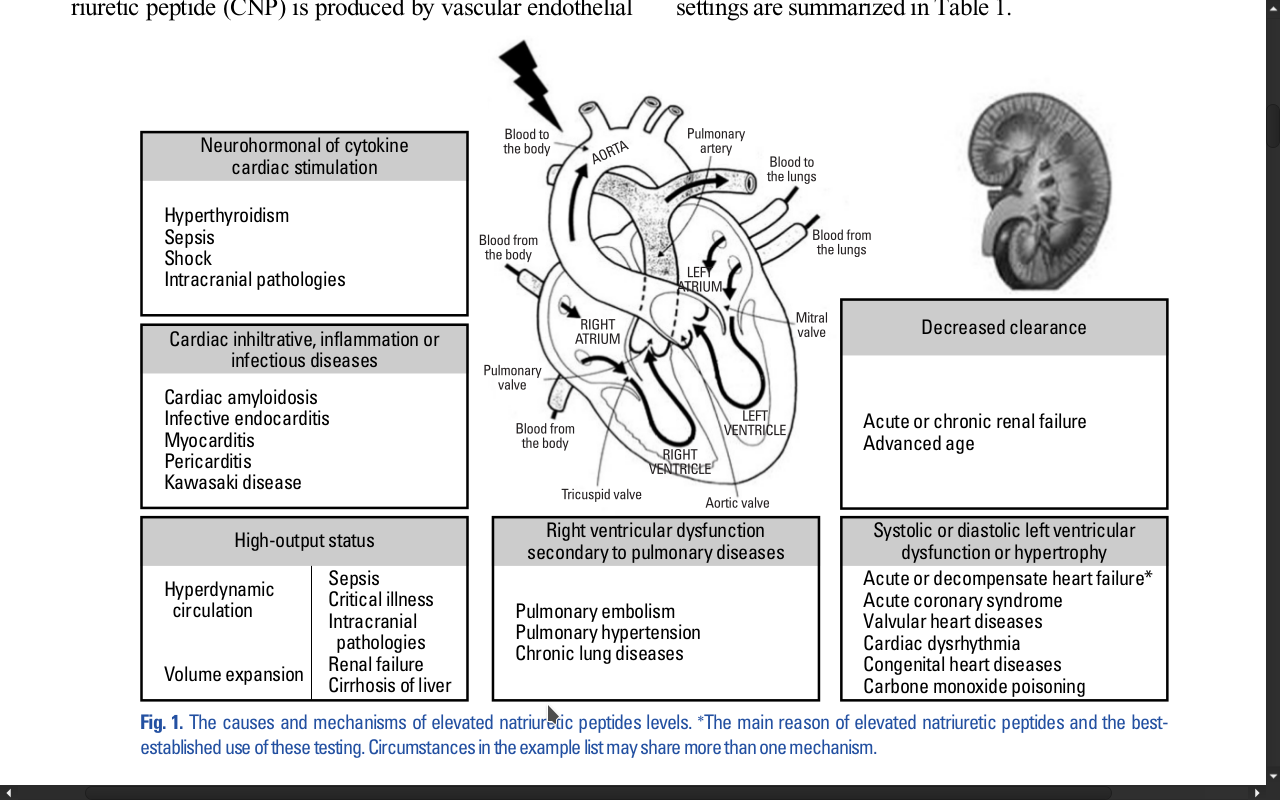
\includegraphics[scale=0.3]{./images/NP_causes.png}
    \caption{The causes and mechanisms of elevated natriuretic peptides levels.}
    \label{NP_causes}
\end{figure}

\begin{table}
    \centering
    \caption{Potential Clinical Applications of Natriuretic Peptides in Selected Diseases}
    \begin{tabular}{|l|c|c|c|}
        \hline
        Diseases & Screening \footnote{Screening for the presence of cardiac dysfunction} &  & Prognosis \\
        \hline
        Heart failure \footnote{The best-established clinical application of these natriuretic peptides testing} & + & + & + \\
        Acute coronary syndrome & + & + & + \\
        Cardiac procedures & + & + & + \\
        Pulmonary embolism & + & + & + \\
        Pulmonary hypertension & + & + & - \\
        Chronic lung diseases & + & + & + \\
        Valvular heart diseases & + & + & N/A \\
        Cardiac dysrhythmia & + & + & +/- \\
        Cardiac inflammatory or infectious diseases & + & + & N/A \\
        Cardiogenic syncope & + & N/A & N/A \\
        Sleep apnea & + & + & N/A \\
        Hypertension & + & + & N/A \\
        Sepsis & + & + & + \\
        Renal failure & + & + & + \\
        Cirrhosis of liver & + & + & + \\
        Hyperthyroidism & + & + & N/A \\
        Intracranial pathologies & + & + & + \\
        Epilepsy / Seizures & + & - & - \\
        Carbone monoxide poisoning & + & N/A & N/A \\
        \hline
    \end{tabular}
    \label{NP_applications}
\end{table}


\subsubsection{B-Type Natriuretic Peptide}
BNP was initially purified and sequenced from extracts of porcine brain tissue and hence it was named brain natriuretic peptide \citep{Sudoh1988}. Subsequently, BNP was found at much higher concentrations in cardiac tissues \citep{Mukoyama1991} \citep{Mukoyama1990}.

%PreproBNP is 134 amino acids in length, consisting of a 26 amino acid signal sequence followed by 108 amino acids that constitute proBNP. Unlike preproANP, which has high species homology throughout the entire polypeptide sequence, preproBNP sequences in mammals only have high homology at the amino and carboxyl terminal ends of the polypeptide. For example, the homology of canine preproBNP to human preproBNP is 53\%, whereas the homology for preproANP between these species is 85\%. This lower level of homology gives rise to differing lengths of the active, circulating BNP between mammalian species. For example, in humans and pigs circulating BNP is 32 amino acids in length, while in rats and mice the circulating form is 45 amino acids. The peptidase that cleaves proBNP to its active form has not been identified, but corin is a reasonable suspect.

Although low levels of BNP are stored with ANP in atrial granules, BNP is found at greater concentrations in cardiac ventricles. In this tissue, BNP is not stored in granules, but rather transcribed as needed in response to cardiac stress states. \citep{Grepin1994} \citep{Thuerauf1994} In normal human subjects, plasma concentrations of BNP are very low (1 fmol/ml), but in response to congestive heart failure, circulating concentrations of BNP are dramatically elevated \citep{Mukoyama1991} \citep{Mukoyama1990}.

BNP can be produced in both atria and ventricles, and is upregulated in failing ventricular myocardium. In response to increased myocardial stretch and wall stress, ventricular myocytes secret the pro-hormone pre-proBNP, which is then cleaved into biologically active BNP and the inactive byproduct N-terminal-proBNP (NT-proBNP). Elevated BNP levels have been demonstrated to be a response to increased angiotensin II and sympathetic tones. \citep{Iwanaga2006}


BNP is eliminated by binding to the NPR-C or degradation by NEP on endothelial cells, smooth muscle cells, cardiac myocytes, renal epithelium, and fibroblasts. NT-proBNP is cleared mainly by the kidney.\citep{Schrier1999}  Compared to ANP, circulating BNP has a significantly longer half-life of around 20 min in humans \citep{Mukoyama1991} \citep{Mukoyama1990}; the half-life of NT-proBNP is about 60-90 minutes and would be expected to be longer in the setting of renal dysfunction. Unlike ANP, BNP is not initially cleaved by NEP. Instead, the first six amino-terminal amino acids of BNP are first cleaved by the metalloprotease, meprin A in the kidney brush border, which then allows further degradation by NEP \citep{Pankow2007}. % Obese patients tend to have lower BNP levels than others. Neural endopeptidases that can be secreted by adipose tissue may be related to increased BNP clearance in obese patients.\citep{Yang2004}

Plastic tubes containing ethylenedinitrolotetraacetic acid (EDTA) are desirable for BNP determination and refrigeration is required if the interval between blood collection and analysis is over 4 hours; whereas NT-proBNP can be measured in both serum or plasma, collected in glass or plastic tubes, and has no significant loss of immunoreactivity after 48 hours at room temperature. Although these existing BNP assays correlate closely, BNP assays are not currently analytical equivalent due to lack of assay standardization.\citep{Omland2008}  A multicenter colloborative proficiency testing study conducted in 90 Italian laboratories had demonstrates that there are significant differences in analytical characteristics and measured values among the most popular commercial methods for BNP and NT-proBNP. Thus, clinicians should be very careful when comparing results obtained by laboratories that use different methods.\citep{Prontera2009}

%Both knockout and overexpression models of NPPB have been generated in mice. The knockout model of Nppb was created by targeted deletion of exons 1 and 2 \citep{Tamura2000}. In contrast to ANP knockout mice, Nppb -/- mice showed no signs of systemic hypertension or ventricular hypertrophy on standard or high salt diets. However, Nppb -/- mice had ventricular fibrotic lesions that increased in size and number in response to pressure overload, compared to wild type animals. Thus, these studies suggest that BNP is not a regulator of blood pressure, at least in mice. Rather, it is a paracrine regulator of cardiac remodeling. In murine overexpression models of BNP, blood pressure reduction of 20 mmHg was seen with 10- to 100-fold increases in plasma BNP levels \citep{Ogawa1994a}. Interestingly, these mice had marked increases in long bone length compared to their wild-type littermates, which most likely resulted from overactivation of NPR-B, the receptor of CNP

\subsubsection{C-Type Natriuretic Peptide}
C-type natriuretic peptide (CNP) was initially purified and sequenced from porcine brain extracts \citep{Sudoh1990}. It is the most highly expressed natriuretic peptide in the brain but is also highly expressed in chondrocytes and endothelial cells. Unlike ANP and BNP, the human gene encoding CNP, NPPC, is not located on chromosome 1 but on chromosome 2 \citep{Ogawa1994b}.

%NPPC encodes a polypeptide of 126 amino acids, with a 23 amino acid signal sequence followed by a 103 amino acid proCNP \citep{Tawaragi1991}. PreproCNP shows remarkable homology between species, even more so than preproANP. The preproCNP polypeptides of mammalian species show 99, 96, 91, and 94\% homology to the human form in chimpanzees, dogs, mice, and rats, respectively. Perhaps even more telling is that the circulating 22 amino acid carboxyl terminal form of CNP is absolutely identical in all of the above species.

Processing of proCNP to its mature form may occur through the action of the intracellular serine endoprotease, furin. In vitro, furin cleaves the 103 amino acid proCNP into a 53 amino acid carboxyl-terminal biologically active peptide \citep{Wu2003a}. This 53 amino acid form of CNP (CNP-53) is the major active form of CNP, at the tissue level \citep{Brown1997}. However, in the systemic circulation, a shorter 22 amino acid form dominates (CNP-22). The protease responsible for this cleavage is not known. Importantly, CNP-53 and CNP-22 appear to bind and activate their cognate receptor, NPR-B, equally well \citep{Yeung1996}.

CNP is not stored in granules and its secretion is increased by growth factors \citep{Suga1993} \citep{Suga1992b} and sheer stress \citep{Chun1997} in cultured endothelial cells. CNP expression in neo-intimal vascular smooth muscle cells is increased in response to vascular injury \citep{Brown1997}. In normal human subjects, mean CNP concentration is very low (1 fmol/ml). It is elevated in patients with congestive heart failure, although to a much lower extent than ANP and BNP \citep{Charles2006} \citep{Del-Ry2005} \citep{Kalra2003}.

\subsection{Natriuretic Peptide Receptors}
There are three known natriuretic peptide binding proteins. All members contain a relatively large (\~450 amino acid) extracellular ligand binding domain and a single membrane-spanning region of about 20 residues. Natriuretic peptide receptors A and B contain an equally large intracellular domain consisting of a so-called kinase homology domain, dimerization domain, and carboxyl-terminal guanylyl cyclase domain. Thus, NPR-A and NPR-B signal by catalyzing the synthesis of the intracellular signaling molecule cGMP. In contrast, NPR-C only contains a 37 residue intracellular domain and lacks guanylyl cyclase activity. It primarily controls local natriuretic peptide concentrations via receptor-mediated internalization and degradation, although many groups have reported signaling functions for NPR-C as well \citep{Rose2008}.

\begin{figure}
    \centering
    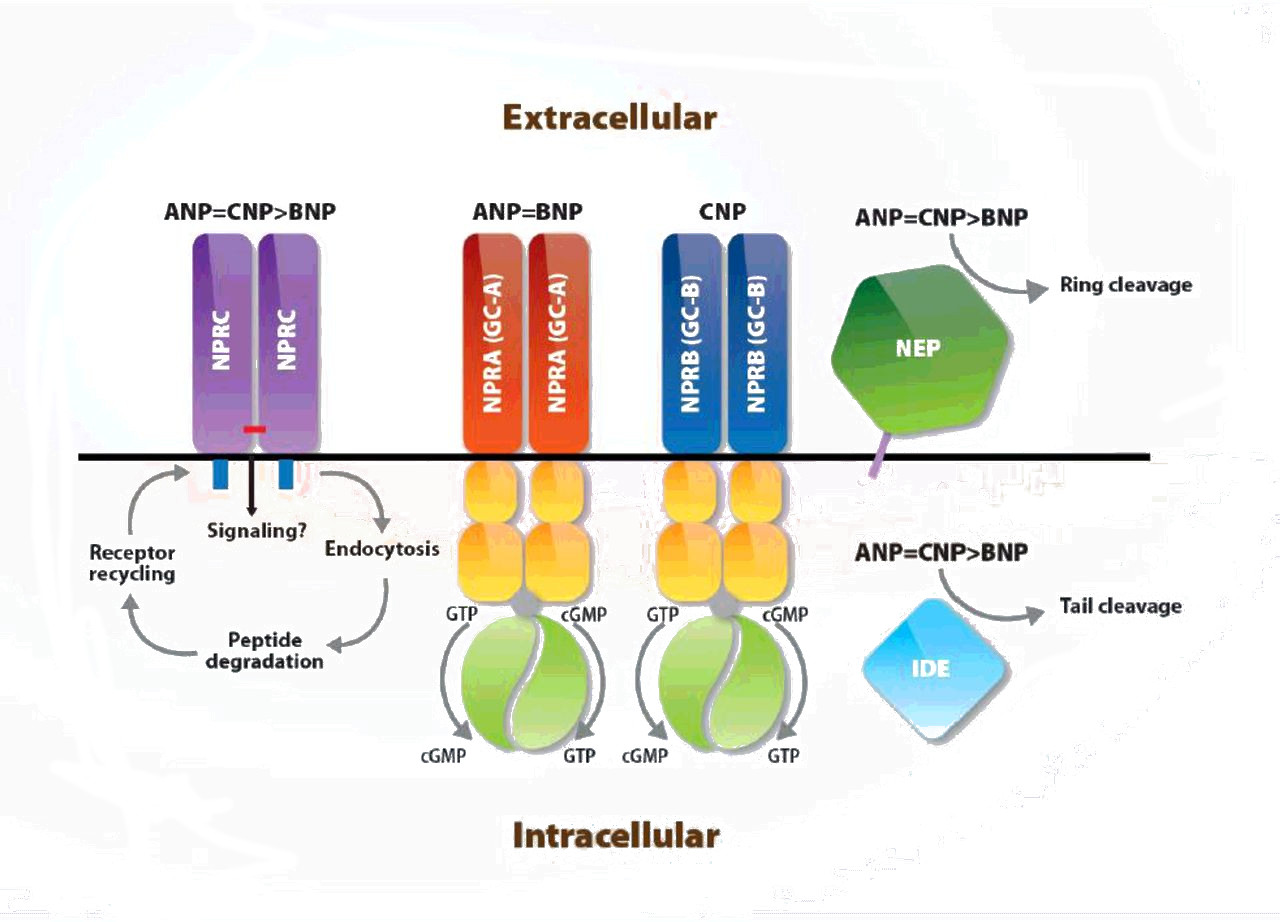
\includegraphics[scale=1]{./images/NP_receptors.jpg}
    \caption{Schematic representation of natriuretic receptors}
    \label{NP_receptors}
\end{figure}


\subsubsection{Natriuretic Peptide Receptor-A}
Natriuretic peptide receptor-A (NPR-A) is the principal receptor of ANP and BNP.
%Its extracellular domain contains three intramolecular disulfide bonds and five N-linked glycosylation sites \citep{Miyagi2000a}.  NPR-A exists as a homodimer or homotetramer in its native state, and oligomerization is ligand-independent \citep{Chinkers1992} \citep{Iwata1991}, although ligand binding does bring the juxtamembrane regions of each monomer closer together \citep{Labrecque2001}.
NPR-A binds natriuretic peptides at a stoichiometry of 2:1 with a rank natriuretic peptide preference of: ANP $\ge$ BNP $>$ CNP \citep{Bennett1991} \citep{Koller1991} \citep{Suga1992a}.

Phosphorylation is essential for activation of NPR-A and dephosphorylation is a mechanism of desensitization in response to prolonged ANP exposure or protein kinase C activation \citep{Potter1992} \citep{Potter1994}. Although ATP increases ANP-dependent guanylyl cyclase activity, the mechanism for this effect is debatable \citep{Antos2005} \citep{Antos2007} \citep{Burczynska2007} \citep{Joubert2005}.  Data indicate that ATP reduces the Km for NPR-A \citep{Antos2007}.

NPR-A internalization and degradation is also controversial. One group consistently reports that the majority of internalized ANP-NPR-A complexes are degraded via a lysosomal pathway with a small portion returning intact to the plasma membrane \citep{Pandey2002}. Meanwhile, studies in primary kidney and Chinese Hamster ovary indicate that NPR-A is a membrane resident protein that does not undergo acute internalization and degradation \citep{Fan2005} \citep{Koh1992} \citep{Vieira2001}.

NPR-A and/or its mRNA is expressed in kidney, lung, adipose, adrenal, brain, heart, testis, and vascular smooth muscle tissue \citep{Goy2001}. NPR-A null mice exhibit chronic salt-resistant hypertension and cardiac hypertrophy and fibrosis \citep{Kuhn2002}.  A deletion in the human NPR-A gene was identified in nine Japanese individuals, of which eight had essential hypertension; the normotensive individual with the altered allele had left ventricular hypertrophy \citep{Nakayama2000}.  %To our knowledge, this study has not been repeated.

\subsubsection{Natriuretic Peptide Receptor-B}
Natriuretic peptide receptor-B (NPR-B) is the principal receptor of C-type natriuretic peptide (CNP) and exhibits similar topology, glycosylation, and intramolecular disulfide bonding patterns as NPR-A.
%The extracellular and intracellular regions of rat NPR-B are 43 and 78\% identical to rat NPR-A at the amino acid level, respectively \citep{Schulz1989}.
NPR-B binds natriuretic peptides with a selectivity preference of CNP $>$ ANP $\ge$ BNP \citep{Bennett1991} \citep{Koller1991} \citep{Suga1992a}.

NPR-B dephosphorylation has been shown to mediate desensitization in response to prolonged CNP exposure, protein kinase C activation, and intracellular calcium elevations \citep{Potter1998} \citep{Potter2000} \citep{Potthast2004}. ATP increases the guanylyl cyclase activity of NPR-B, by decreasing its Michaelis constant \citep{Antos2007}.
NPR-B and/or its mRNA is expressed in bone, brain, fibroblasts, heart, kidney, liver, lung, uterine, and vascular smooth muscle tissue \citep{Bryan2006} \citep{Dickey2007}. Mice with a targeted disruption of the NPR-B gene, display dwarfism and  female sterility \citep{Tamura2004}.

NPR-B dominant negative mutant transgenic rats have also been generated \citep{Langenickel2006}. In addition to mild growth retardation of the long bones, the rats displayed progressive, blood pressure-independent cardiac hypertrophy and an elevated heart rate.

Consistent with a prominent role for CNP in the heart, NPR-B, not NPR-A, is the most active natriuretic peptide receptor in the failed heart \citep{Dickey2007}. Homologous loss-of-function mutations in human NPR-B result in a rare form of dwarfism called acromesomelic dysplasia, type Maroteaux (AMDM) \citep{Bartels2004}.

\subsubsection{Natriuretic Peptide Receptor-C}
Natriuretic peptide receptor-C (NPR-C) consists of a large extracellular ligand-binding domain that is approximately 30-35\% identical to NPR-A and NPR-B, a single membrane-spanning region, but only 37 intracellular amino acids \citep{Chang1989} \citep{Fuller1988} \citep{Porter1990}. It has no known enzymatic activity but has been  suggested to signal in a G protein-dependent manner \citep{Rose2008}.
It binds natriuretic peptides with a stoichiometry of two molecules of receptor to one molecule of ligand \citep{Ammarguellat2001}. Its ligand selectivity preference is: ANP $>$ CNP $\ge$ BNP \citep{Bennett1991} \citep{Suga1992a}.

The main function of NPR-C, also known as the clearance receptor, is to clear circulating natriuretic peptides through the process of receptor-mediated internalization and degradation \citep{Koh1992} \citep{Nussenzveig1990}. Internalization of NPR-C occurs in the absence of ligand; thus, this is a constitutive process \citep{Nussenzveig1990}. Osteocrin, an endogenous protein with limited homology to members of the natriuretic peptide family, binds NPR-C, but not NPR-A or NPR-B \citep{Moffatt2007}. Osteocrin is thought to compete with CNP for binding to NPR-C in bone, and therefore, increase local CNP levels during critical periods for bone development \citep{Moffatt2007}.

NPR-C is the most widely and abundantly expressed natriuretic peptide receptor; for example, it constitutes \~94\% of the total ANP binding sites in endothelial cells \citep{Leitman1986}. NPR-C and/or its mRNA is expressed in adrenal, brain, heart, kidney, mesentery, and vascular smooth muscle tissue \citep{Nagase1997} \citep{Porter1990} \citep{Suga1992c} \citep{Wilcox1991}.
NPR-C knockout mice exhibit increased ANP half-lives, long bone overgrowth, hypotension, mild diuresis, dilute urine, and blood volume depletion  \citep{Matsukawa1999}. Mouse strains containing chemically induced loss-of-function mutations in the extracellular domain of NPR-C display skeletal overgrowth from endochondral ossification defects as well \citep{Jaubert1999}.

\subsection{Physiologic Effects of Natriuretic Peptides}


\subsubsection{Natriuretic Peptide Effects on Blood Pressure}
ANP binding to NPR-A is a key-signaling pathway, which regulates normal homeostatic blood pressure. This is clearly demonstrated in mice lacking ANP or its receptor NPR-A, which have blood pressures that are elevated 20-40mmHg, compared to control mice \citep{John1995} \citep{John1996} \citep{Lopez1995} \citep{Oliver1997}.
The link between NPR-A and blood pressure in mice is particularly strong because Smithies and colleagues demonstrated that NPR-A copy number is inversely related to blood pressure in a  remarkably linear manner \citep{Oliver1998}.
Conversely, blood pressures in transgenic mice overexpressing ANP or BNP are substantially decreased \citep{Ogawa1994a} \citep{Steinhelper1990}. Although infusion of supraphysiological levels of CNP into animals acutely decreases blood pressure \citep{Clavell1993} \citep{Sudoh1990}, mice lacking functional CNP or NPR-B are normotensive \citep{Chusho2001} \citep{Tamura2004}, suggesting that the CNP/NPR-B pathway is not a fundamental regulator of basal blood pressure in mice.

NPR-A dependent decreases in blood pressure are achieved through natriuresis and diuresis, vasorelaxation, increased endothelium permeability, and antagonism of the renin-angiotensin system. Classic experiments showed that atrial extract infusions resulted in rapid renal excretion of water and sodium \citep{deBold1981}. Studies by Garbers and colleagues indicated that the renal response requires NPR-A because mice lacking this receptor do not respond to ANP, BNP, or to acute volume expansion \citep{Kishimoto1996}. Similar studies found that NPR-A was also required for ANP- or BNP-dependent vasorelaxation in mice \citep{Lopez1997}. Physiological experiments involving mice with severe reductions of NPR-A in vascular smooth muscle cells demonstrated that while smooth muscle NPR-A is required for acute ANP- or BNP-dependent vasorelaxation, this response does not play a significant role in controlling chronic blood pressure \citep{Holtwick2002}.

The ability of the ANP/NPR-A pathway to increase  endothelial permeability is supported by the observation that hematocrit levels are elevated prior to urination and are preserved in nephrectomized animals \citep{Almeida1986} \citep{Fluckiger1986} \citep{Richards1988}.
 Furthermore, mice with genetically engineered reductions of NPR-A in vascular endothelium exhibit volume expansion, hypertension, and reduced albumin clearance from the vascular system \citep{Sabrane2005}.

\subsubsection{Effects of Natriuretic Peptides on Cardiac Hypertrophy and Fibrosis}

Although prolonged hypertension can cause hypertrophy, the level of hypertrophy in NPR-A deficient mice is significantly greater than that observed in other genetic models that cause similar levels of hypertension, suggesting that NPR-A elicits a local growth inhibitory signal in the heart. Data for this idea was initially shown in NPR-A knockout mice, which have enlarged hearts even when effectively treated with antihypertensive drugs from birth \citep{Knowles2001}. Additional studies determined that transgenic re-expression of NPR-A in the hearts of NPR-A -/- mice reduced cardiomyocyte size without affecting heart rate or blood pressure \citep{Kishimoto2001}.
Finally, mice with reduced cardiomyocyte expression of NPR-A exhibited moderate hypertrophy even though they were slightly hypotensive \citep{Holtwick2003} \citep{Patel2005}. In terms of natriuretic peptides, mice lacking ANP have larger hearts, whereas mice transgenically overexpressing ANP have smaller hearts \citep{Barbee1994} \citep{Steinhelper1990}.
In contrast, targeted deletion of BNP resulted in normotensive mice with normal heart size but with increased ventricular fibrosis - especially when subjected to pressure overload \citep{Tamura2000}. Thus, genetic studies in mice strongly support a role for ANP activation of NPR-A in the local inhibition of cardiac hypertrophy and BNP activation of NPR-A in the inhibition of cardiac fibrosis.

Data supporting a role for the CNP/NPR-B pathway in cardiac remodeling has been reported. Although NPR-B inactivation mutations in mice have not been shown to cause hypertrophy \citep{Tamura2004} \citep{Tsuji2005}, transgenic rats expressing a dominant negative form of NPR-B exhibit mild blood pressure-independent cardiac hypertrophy and increased heart rate \citep{Langenickel2006}.
In addition, CNP infusion was shown to reduce cardiac remodeling in response to experimentally induced myocardial infarction in rats, and transgenic expression of CNP improved outcomes in mice subjected to ischemia/reperfusion injury or myocardial infarction \citep{Wang2007}.

\subsubsection{Effects of CNP and NPR-B on Bone Growth}
The most obvious function of the CNP/NPR-B pathway is to stimulate long bone growth. Though undetectable at birth, mice lacking functional CNP or NPR-B develop dwarfism due to impaired endochondrial ossification \citep{Chusho2001} \citep{Tamura2001} \citep{Tsuji2005}.
Conversely, transgenic CNP overexpression or reduced degradation of CNP due to loss-of-function mutations in NPR-C result in skeletal overgrowth \citep{Jaubert1999} \citep{Matsukawa1999}  \citep{Yasoda2004}. Growth plate histology reveals that the endochondral proliferative and hypertrophic zones are reduced in mice with impaired CNP or NPR-B signaling, whereas overexpressing mice have enlarged growth plates \citep{Chusho2001} \citep{Tamura2004} \citep{Yasoda2004}.

One cGMP effector involved in the long bone growth pathway is cGMP-dependent protein kinase II, also known as PKGII or cGKII. Loss-of-function mutations in the mouse or rat gene that encodes this kinase also cause dwarfism \citep{Chikuda2004} \citep{Pfeifer1996}. Interestingly, the growth plates of rodents with defective cGKII are enlarged, which differs from the diminished growth plates seen in the CNP or NPR-B deleted mice, suggesting that a cGKII-independent pathway is also involved in CNP-dependent long bone growth.

Humans with two loss-of-function alleles for NPR-B suffer from a rare type of autosomal recessive dwarfism, called acromesomelic dysplasia, type Maroteaux \citep{Bartels2004}. These individuals are characterized by disproportionate limb to torso ratios that are only obvious a year or more after birth. Interestingly, although single copy carriers of a nonfunctional NPR-B allele do not suffer from disease, they are statistically shorter than comparable individuals with two wild type NPR-B alleles \citep{Olney2006}. Thus, it is possible that NPR-B mutations could have a significant effect on the stature of the general population.

\subsection{Therapeutics of Natriuretic Peptides}

Measurement of serum BNP levels is used in the clinic as a diagnostic indicator for heart failure, and synthetic forms of both ANP and BNP have been approved in some countries for the treatment of heart failure \citep{Gardner2003a}. The extent of their usefulness, however, has come under question due to their limited renal actions, and trials are underway to determine the most effective use of these peptides. In this section, we will explore the history of both synthetic ANP and BNP as therapeutic agents. %TO-DO search for more recent data

\subsubsection{Synthetic ANP (Anaritide and Carperitide)}
Studies revealed that the mature form of ANP is a 28-amino-acid peptide and that smaller versions are degradation products that maintain various levels of activity. The most widely studied of these is the 25-amino acid peptide lacking the first three amino-terminal residues. This peptide is referred to as ANF IV and its synthetic form is called anaritide.
Since the activities of the 25-amino acid and mature 28-amino acid peptide were similar, many studies were conducted with the smaller peptide. Studies by Cody and colleagues indicated that infusion of anaritide in healthy male volunteers resulted in natriuresis, diuresis, and reduction in systolic blood pressure; however, in seven patients with congestive heart failure, the changes in urine volume and sodium excretion were minimal \citep{Cody1986}. Saito and colleagues observed a similar lack of diuresis and natriuresis, when congestive heart failure patients were infused with the mature form of ANP \citep{Saito1987}.

Meanwhile, others acknowledged the renal hyporesponsiveness to anaritide in congestive heart failure patients, but indicated that the renal parameters did show a statistically significant increase in larger patient samples \citep{Fifer1990}. In Japan, clinical studies on the effectiveness of mature ANP continued; and in 1995, synthetic full length ANP (carperitide) was approved for the treatment of acute decompensated heart failure. In the United States, clinical use of BNP, not ANP, was explored for the treatment of heart failure due to its larger renal responsiveness, and possibly due to unique patient opportunities. %TO-DO lacking reference!

Investigations were also initiated to study the effectiveness of ANP in the treatment of human renal disease. Specifically, trials were conducted to evaluate the ability of anaritide infusion to reduce the need for dialysis in patients with acute tubular necrosis. The initial study with 53 patients suggested a positive outcome for patients receiving anaritide because they had increased creatinine clearance and a decreased need for dialysis \citep{Rahman1994}. This led to the formation of a multicenter placebo-controlled clinical trial in 504 patients with acute tubular necrosis. While 24-h infusion of anaritide did not improve the overall survival of the patients without dialysis, it appeared that a subset of patients might have benefited \citep{Allgren1997}.
Thus, a second trial was conducted in patients with oliguric acute renal failure. However, this 222 patient trial indicated no statistically significant benefit of anaritide in dialysis-free survival \citep{Lewis2000}. Both trials remarked on the severe hypotension that often occurred as a result of the anaritide infusion. In fact, it is this severe hypotension that appears to be limiting the utility of anaritide or nesiritide as a therapy for either heart failure or renal disease. The authors stated in their discussion, it is possible that if this hypotension could have been avoided, anaritide would have been efficacious \citep{Lewis2000}.  Anaritide was also investigated for its ability to prevent radiocontrast-induced nephropathy. However, in a 247 person clinical trial anaritide along with hydration was no more effective at preventing radiocontrast-induced nephropathy than hydration alone \citep{Kurnik1998}.

Finally, in 2004, studies conducted in Sweden compared the ability of the loop diuretic, furosemide, or mature ANP (1-28) to increase GFR, renal blood flow, and reduce renal oxygen consumption in patients with acute renal failure. They concluded that furosemide was a more effective agent \citep{Sward2005}. Therefore, despite its potent natriuretic and diuretic effects in normal, healthy subjects, clinical studies conducted to date indicate little or no therapeutic benefit of ANP analogs in the successful treatment of renal disease.

\subsubsection{Synthetic BNP (Nesiritide)}
Given the natriuretic effects of ANP, the related peptide BNP, was assumed to elicit a similar response. McGregor and colleagues demonstrated that administration of porcine BNP resulted in a natriuretic response and an increase in urinary excretion of cGMP \citep{McGregor1990}. Yoshimura and colleagues reported the same response in healthy volunteers to infusion of human BNP \citep{Yoshimura1991}.

Patients with congestive heart failure also responded to infusion of BNP.  The effectiveness of 24-h infusion of nesiritide to patients with congestive heart failure was examined in a multicenter, placebo-controlled trial. The peptide resulted in a reduction of both preload and afterload resulting in an increase in stroke volume and cardiac output \citep{Mills1999}.
The results of a second multicenter trial, called the Vasodilation in the Management of Acute Congestive Heart Failure (VMAC) study, compared the effects of the addition of nitroglycerin or nesiritide versus placebo to standard therapy. The group treated with nesiritide had improved dyspnea after 3 h treatment, while there was no difference in the other groups. The nitroglycerin group reported more adverse effects than the nesiritide group. Additionally, patients receiving nesiritide had less adverse cardiovascular effects at either the 0.015 or 0.03mcg/kg/min infusion rate compared to patients receiving dobutamine as determined by the 246-patient PRECEDENT Trial \citep{deLissovoy2003}.  % TO-DO study the VMAC and PRECEDENT trials

With the approval of the first new intravenous compound for the treatment of heart failure in many years, use of nesiritide was immediate. After approval, the number of patients treated with nesiritide was larger than any clinical trial and with the larger sample population came some unpleasant findings. Initially, Wang and colleagues reported in 2004 that nesiritide does not improve renal function in patients with chronic heart failure \citep{Wang2004a}, but more damaging were two meta-analysis studies by Sackner-Bernstein and colleagues indicating that nesiritide worsened renal function and increased the likelihood of death \citep{Sackner-Bernstein2005a} \citep{Sackner-Bernstein2005b}. % TO-DO stugy them

The results of a 75-person study (BNP-CARDS study), however, suggest nesiritide has no detrimental effect on renal function, when cohorts of similar baseline renal function were compared \citep{Witteles2007}. The number of persons in this study was small, however, so a more definitive conclusion on whether nesiritide impairs renal function will have to wait until the result of more detailed, larger studies are released. Several such studies are currently in progress. One is a clinical trial enlisting at least 1,900 patients throughout Europe and Latin America - the ETNA (Evaluating Treatment with Nesiritide in Acute Decompensated Heart Failure) trial.
This trial was scheduled to begin in 2006 to study the efficacy of nesiritide on treatment of acutely decompensated heart failure. Results from the trial are not yet available. The second study involving about 900 patients, called FUSION II, was conducted to determine the safety and efficacy of outpatient administration of nesiritide to patients with heart failure. Preliminary analysis indicates that nesiritide did not induce renal complications or increase patient mortality \citep{Cleland2007}. %TO-DO find more recent data

Finally, there is the ASCEND HF trial (Acute Study of Clinical Effectiveness of Nesiritide in Decompensated Heart Failure). This trial is scheduled to compare the effects of nesiritide treatment versus placebo for a minimum of 24 h up to a maximum of 7 days in 7,000 heart failure patients. Meanwhile, other therapeutic applications of nesiritide have also been investigated. Given that nesiritide was often reported to decrease pulmonary capillary wedge pressure, Michaels and colleagues tested its effectiveness in pulmonary hypertension, however, they found no effect for a 30 min infusion \citep{Michaels2005}. Chen and colleagues have investigated the effectiveness of subcutaneous injections of nesiritide. Their most recent paper on effects in a dog heart failure pacing model suggest that subcutaneous injection of nesiritide reduces both preload and afterload but has no effect on cardiac output \citep{Chen2006}.

\subsection{BNP and NT-proBNP}
\subsubsection{Differences in Physiology}
BNP is a hormonally active natriuretic peptide that is mainly released from the cardio-myocytes in the left ventricular wall. In reaction to stretch and tension of the myocardial wall the pro-hormone proBNP splits into BNP and the hormonally inactive remnant N-terminal proBNP (NT-proBNP) by proteolytic cleavage Fig. \ref{BNP_secretion}. \citep{Pfister2004} This process occurs under influence of integrins, structures at the Z-disc of sarcomeres, that measure stretch of these sarcomeres \citep{Liang2000,Pyle2004} after which both peptides will be secreted in equimolar amounts into the circulation.

Circulating BNP acts as an antagonist of the renin angiotensine aldosterone system, and protects the body from plasma overload by inducing diuresis, natriuresis, vascular dilatation and inhibition of the sympathetic nervous system. \citep{Sudoh1988} The half life of BNP is around 20 minutes and the half life of NT-proBNP is around 120 minutes. BNP is known to be cleared from the blood by natriuretic peptide clearance receptors, by neuro endopeptidases and by the kidneys. Little is known on the exact clearance mechanism of NT-proBNP, although it has been suggested that the kidneys play a major role in this clearance. \citep{Hall2005}
Absolute values of BNP are significantly lower than values of NT-proBNP, despite equimolar secretion. The reference ranges for BNP and NT-proBNP vary depending on the assay that is used and the nature of the control population. In general, the suggested normal range for circulating BNP is 0.5-30 pg/ml and for circulating NT-proBNP the suggested normal range is 68-112 pg/ml. \citep{Cowie2003} These natriuretic peptides may be beneficial in clinical practice since plasma levels of BNP and NT-proBNP are elevated in patients with HF and are related to the severity of the disease. \citep{Mukoyama1990}

\begin{figure}
    \centering
    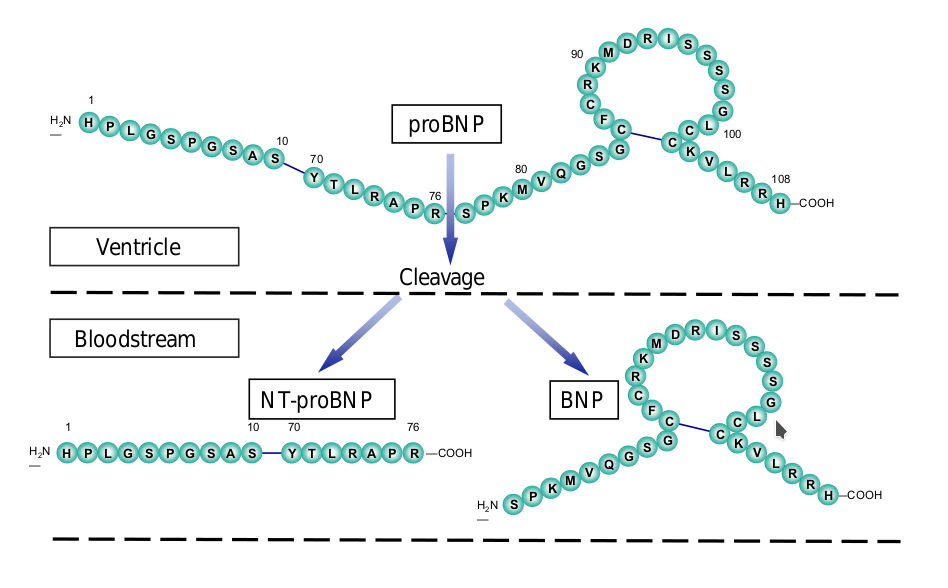
\includegraphics[scale=0.4]{./images/BNP_secretion.png}
    \caption{Secretion of BNP and NtproBNP}
    \label{BNP_secretion}
\end{figure}

\subsubsection{BNP and NT-proBNP in clinical practice}
BNP and NT-proBNP plasma levels are promising tools in the daily management of suspected or established HF. Most studies on the use of BNP and NT-proBNP in clinical practice addressed their diagnostic properties. However, an increasing amount of evidence is available on the prognostic value of BNP and NT-proBNP and some studies provided hopeful results for the benefits of NT-proBNP guided medical treatment.

\textbf{Diagnosis}

Recent trials provided strong evidence that BNP and NT-proBNP are powerful diagnostic tools in exclusion and diagnosis of HF. The Breathing Not Properly study showed, by means of receiver operating characteristics analyses, that a BNP value of 100 pg/ml was the optimal value to differentiate patients with dyspnoea caused by HF from patients with dyspnoea due to pulmonary pathology at the emergency department Fig. \ref{BNP_ER}. \citep{Maisel2002}

This value of 100 pg/ml also discriminated non-systolic HF (LVEF <45\%) from non-HF patients at the emergency department. It has also been suggested that BNP could be used to discriminate systolic from diastolic HF. Although non-systolic HF patients had significantly lower BNP plasma levels than systolic HF patients (LVEF >45\%), BNP only had modest added value in differentiating non-systolic from systolic HF. In another study, a BNP value of 100 pg/ml added significant value to the diagnosis of HF on top of clinical judgement. \citep{McCullough2002}

 An international pooled analysis of 1256 patients provided cut off values for NT-proBNP in an emergency department setting. An age independent cut point of 300 pg/ml had a negative predictive value of 98\%.  Additionally, an optimal strategy to identify acute HF was to use age stratified cut off points of 450, 900 and 1800 pg/ml for ages <50, 50-75, and >75 respectively which yielded 90\% sensitivity and 84\% specificity for acute HF Fig. \ref{NTBNP_ER}. \citep{Januzzi2006,Januzzi2005} Furthermore, BNP and NT-proBNP seem useful as diagnostic tools in primary care (where most patients with suspected HF are encountered and where only limited diagnostic tools are available) and as such are recommended in recent guidelines. \citep{Swedberg2005}

 The added value of these natriuretic peptides on top of established diagnostic tools, including symptoms and signs, has not been properly studied, in particular in relevant subgroups, and currently large studies are underway addressing this issue.  %CHECK
  Discharge diagnoses have been instrumental in providing estimates and time trends in prevalence and incidence of HF. However, previous studies in the Netherlands, Sweden and in the United States showed that respectively 20\%, 18\% and 33\% of the patients that were given the discharge diagnosis ‘HF’ at close examination did not have HF at all. \citep{Heerdink1995,Ingelsson2005,Goff2000} It is unknown whether the established BNP cut off value of 100 pg/ml can also be used at discharge after admission for HF.

\begin{figure}
    \centering
    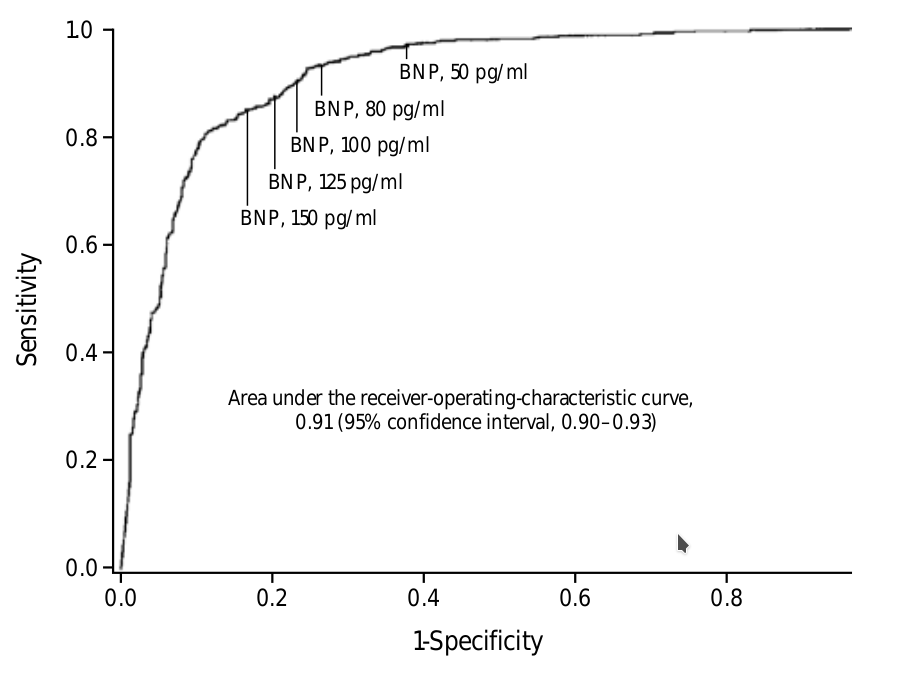
\includegraphics[scale=0.4]{./images/BNP_ER.png}
    \caption{ROC curves for BNP in the diagnosis of heart failure at the emergency department.}
    \label{BNP_ER}
\end{figure}

\begin{figure}
    \centering
    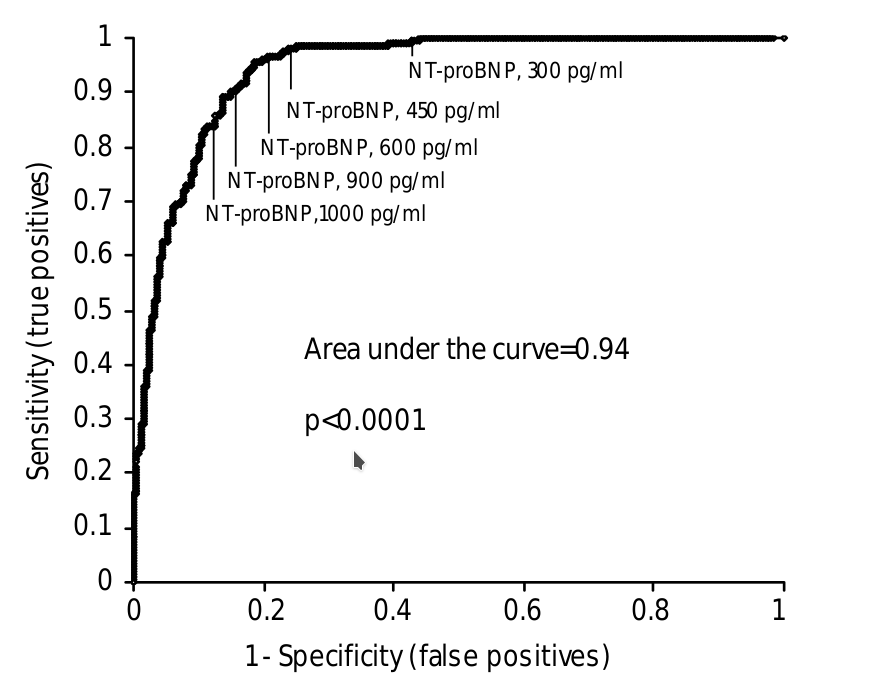
\includegraphics[scale=0.4]{./images/NTBNP_ER.png}
    \caption{ROC curves for NTproBNP in the diagnosis of heart failure at the emergency department.}
    \label{NTBNP_ER}
\end{figure}


\textbf{Prognosis}

The prognostic value of BNP and NT-proBNP is well established in several groups of patients. An early study on 85 patients with chronic HF revealed that BNP is a strong independent predictor of mortality. \citep{Tsutamoto1997} Another study confirmed these results in a larger research population of 452 systolic HF patients (LVEF <35\%). In this study BNP was found to be a strong independent predictor of sudden death during a follow up period of 3 years. \citep{Berger2002}
Furthermore, NT-proBNP was a predictor of sudden death in this study population. A substudy of the COPERNICUS trial (n=1011) revealed that NT-proBNP was consistently associated with an increased risk for all-cause mortality and hospitalisation for HF in patients with severe HF (LVEF <25\%). \citep{Hartmann2004} Another study on 142 patients with advanced HF also reported that NT-proBNP was an independent predictor of all cause mortality. \citep{Gardner2003b}


\textbf{Guidance of treatment}

BNP and NT-proBNP are influenced by drugs that are prescribed to HF patients like diuretics, \citep{Tsutamoto2004} beta blockers, \citep{Richards1999} ACE inhibitors or angiotensine II receptor blockers \citep{Latini2002} and therefore these natriuretic peptides could possibly be used to guide medical treatment. A small study by the Australia-New Zealand Heart Failure Group including 69 patients with symptomatic HF provided evidence of the possible benefit of a NT-proBNP guided approach to therapy. Half of the patients received therapy guided by plasma NT-proBNP, therapy in the remaining patients was guided by clinical monitoring at the same frequency, but with the physician blinded to the NT-proBNP result. Clinical monitoring was based on scores assigned to 10 symptoms or signs of HF used in the Framingham criteria for HF.
The study found significantly lower mortality, fewer hospitalisations and episodes of decompensated HF in the NT-proBNP-guided therapy group (target 1680 pg/ml). \citep{Troughton2000} Larger studies are underway that are about to provide firmer evidence as to whether or not BNP and NT-proBNP can be used as a marker in the monitoring of treatment of HF patients. \citep{Buckley1999} %CHECK

\subsubsection{Variables influencing BNP and NT-proBNP levels: potential limitations?}
Although natriuretic peptide levels are of value in the diagnosis and prognosis of HF patients, several clinical conditions other than HF influence BNP and NT-proBNP plasma levels as well. These influences may be a disadvantage for the use of BNP and NT-proBNP in clinical practice of HF since it may lead to biased interpretations of the test results.

Cardiac variables:
BNP and NT-proBNP are also elevated in patients with acute coronary syndrome. After acute myocardial infarction, levels of BNP rise rapidly during the first 24 hours and then tend to stabilize, \citep{deLemos2001} and in patients with a Q-wave infarction, a peak in NT-proBNP levels was found after 12-48 hours. \citep{Talwar2000} In patients with unstable angina pectoris, BNP levels were found to be four times higher compared to patients with stable angina pectoris. \citep{Kikuta1996}
Moreover, atrial fibrillation resulted in increased BNP levels in patients without, but not in patients with HF. \citep{Knudsen2005} Right ventricular failure due to acute pulmonary embolism can also be determined by BNP. \citep{Tulevski2002} Furthermore, hypertensive patients have higher BNP and NT-proBNP levels compared to non-hypertensive subjects. \citep{Boomsma2001}

Non-cardiac variables:
A few studies in relatively small study populations without HF showed that anaemia causes elevated BNP levels \citep{Tsuji2004,Willis2005,Wold2005} and in a study on a small group of HF patients anaemia was also related to increased NT-proBNP levels. \citep{Wu2005}
However, besides that these studies were limited in sample size, they only investigated one of the two peptides and the effect of anaemia on NT-proBNP was investigated in HF patients only.
Furthermore, anaemia is often caused by renal dysfunction, but this co-morbidity has not been investigated in detail in these studies. Since both BNP and NT-proBNP are known to be elevated in case of renal dysfunction, \citep{Luchner2005} and because renal function and HF are interrelated, a study investigating the effect of anaemia and renal function on both BNP and NT-proBNP in HF patients is needed.
An additional variable that is related to both BNP and NT-proBNP is obesity. In several large studies lower natriuretic peptide levels were associated with higher body mass indexes. \citep{Das2005,Krauser2005,Mehra2004,Wang2004b} As far as diabetes is concerned, results are conflicting between BNP and NT-proBNP; BNP levels did not differ between patients with or without diabetes, \citep{Wu2004} but NT-proBNP levels seem to be higher in diabetic patients compared to non diabetics. \citep{Magnusson2004}
Furthermore, ascitic cirrhosis, hyperaldosteronism, hypercortisolism, carcinoma, subarachnoid hemorrhage, \citep{Pfister2004} lung cancer, tuberculosis and pulmonary embolism \citep{7} are clinical conditions with reported elevated natriuretic peptide levels.

Patient related variables:
Studies showed that both BNP and NT-proBNP levels are influenced by biological variation, with the biological variation of BNP being higher compared to NT-proBNP (up to 44\% and up to 35\% respectively). \citep{Bruins2004,Wu2003b}
Both BNP and NT-proBNP increase with advancing age and are higher in females compared to males in healthy subjects. \citep{Raymond2003} %Nevertheless it is unknown whether there are differences in the age and gender dependency between the two peptides and only limited data are available on the age dependency of BNP and NT-proBNP in HF patients. Furthermore, before BNP and NT-proBNP were discovered, Atrial Natriuretic Peptide (ANP) and N-terminal ANP (NT-ANP), natriuretic peptides that are mainly produced in the atria and with properties comparable to BNP and NT-proBNP, were studied. Although evidence is available on the superiority of BNP over ANP in the diagnosis of HF and of BNP/ NT-proBNP over ANP/ NT-ANP in the prognosis after myocardial infarction, it is unknown which peptide is influenced most by age and gender.

Previous research shows that BNP is related to maximal exercise performance. \citep{Kruger2002} Moreover, the influence of moderate physical activity (75\% of the maximum) on BNP levels was investigated in 10 healthy subjects, 10 HF patients with NYHA class I-II and in 10 HF patients with NYHA class III-IV. A significant increase in BNP levels was observed directly after exercise. \citep{McNairy2002} However, it is not known whether B-type natriuretic peptide levels also reflect sub-maximal functional capacity during daily activities and whether they are related to quality of life.


% \subsection{Coronary Artery Disease}
% An extremely short chapter.  No time to be wasted on it.
%
% \subsection{Coronary Artery Bypass Grafting}
% Also short
% \subsubsection{on-pump vs OPCAB}


\clearpage
\section{Material and Methods}


60 cases registered for elective off-pump coronary artery bypass grafting OPCAB were recruited in this study. Patients were interviewed preoperatively for history taking and clinical examination. EuroScore II was calculated. Demographic, past medical and surgical history, medications and baseline laboratory results (labs. on admission to hopsital) and preoperative angiography results were recorded.  No specific attempts were made to standardize the anesthetic and surgical management.  Venous samples for measuring NT-proBNP were collected on the day of surgery before induction. Samples were sent for analysis in Cairo University Clinical Pathology department. Intra-operative and postoperative data were recorded, including: duration of surgery, number of grafts, intraoperative blood transfusion and, in case CPB was need arotic cross clamp time, CPB time : lowest naso-pharyngeal temp on CPB.  Patients were followed during their hospital stay \footnote{whenever we mention ICU or hospital stay, we mean postoperative duration in ICU and postoperative duration till discharge respectively} and events recorded including: death from cardiovascular causes, ischemic stroke , low output heart failure,  myocardial infarction, prolonged intubaton and arrhythmias.

\subsubsection{Exclusion Criteria}

Patients with signicant valvular heart disease, dilated or hypertophic cardiomyopathy, NYHA III or IV, EF $< 40\%$, preoperative atrial fibrillation, inotropic support or intra-aortic balloon pump, creatinine clearance $< 60$ ml/min/1.73 m2, hyperthyoidism and hypothyroidism, and moderate to severe COPD were excluded to eliminate potential confounding factors which may influence heart function and plasma biomarkers.

Hyperthyroidism and hypothyroidism are defined as serum TSH levels above or below reference ranges respectively.  It was measured only upon clinical suspicion.

\subsubsection{Definitions}
The following definitions were used in this Study
    \begin{description}
        \item [Moderate to severe COPD]
        Shortness of breath at own pace on the level, FEV1 $< 80\%$ of predicted, or continuous use of bronchodilators for $> 2$ weeks.
        \item [ischemic cerebral stroke]
        New neurologic deficit lasting for  24hours with definite image evidence of cerebrovascular accident by computed tomography
        \item [low output heart failure]
        Need of CPB during surgery, intra-aortic balloon pump and/or inotropes at 48 hours post-operatively
        \item [Myocardial infarction]
        Elevated tropoponin 10x99th percentile URL at 12 hours after surgery associated with characteristic ECG changes or echocardiographically documented new regional wall motion abnormality
        \item [Prolonged intubation]
        Intubation more then 24 hours postoperatively and/or reintubation following planned extubation
    \end{description}

\subsubsection{Primary and Secondary Outcomes}
Primary outcomes:
    \begin{itemize}
        \item low output heart failure and myocardial infarction
    \end{itemize}

Secondary outcome parameters:
    \begin{itemize}
        \item mortality
        \item arrhythmias
        \item length of ICU and hospital stay
        \item prolonged intubation
    \end{itemize}

\subsubsection{Data Analysis and Statistical Methods}
Data were coded and entered using the statistical package SPSS (Statistical Package for the Social Sciences) version 24. Data was summarized using mean, standard deviation, median, minimum and maximum in quantitative data and using frequency (count) and relative frequency (percentage) for categorical data. Comparisons between quantitative variables were done using the non-parametric Mann-Whitney test \citep{Chan_a_2003}. Correlations between quantitative variables were done using Spearman correlation coefficient \citep{Chan_b_2003}.  ROC curve was constructed with area under curve analysis performed to detect best cutoff value of NTproBNP for detection of outcomes. P-values less than 0.05 were considered as statistically significant.

\clearpage
\section{Results}

Patients mean age was $57.4\pm7.3$ years, and 86.4\% were male.  One patient didn't undergo surgery; due to failure to obtain consent. Only two patients died; one of sepsis and the other of respiratory failure. Three required prolonged mechanical ventilation, one of whom was due to delayed recovery from anaesthesia (the only patient suffering from such complication). Three suffered recent onset arrhythmia (3 Atrial fibrillation, One Ventricular Tachycardia) during their ICU stay. One patient was re-admitted to the ICU for atrial fibrillation.  Five patients had low output heart failure, and four had perioperative myocardial infarction. The mean ICU stay was $3.37\pm0.84$ days and mean hospital stay was $6.38\pm1.3$ (range 3-12) days.  The preoperative NTproBNP levels ranged 100-14400 pg/mL, with a mean of 3096.83. It didn't correlate with any of the measured outcome parameters. See tables \ref{Result_relation_parameters} and \ref{Result_correl_parameters}

\begin{table}[]
\centering
\caption{pre-operative characteristics of study patients}
\label{Preop_characteristics}
    \begin{tabular}{cccc}
    \hline
                                           &     & count & \%   \\ \hline

    \multirow{2}{*}{Gender}                & f   & 9     & 13.6 \\
                                           & m   & 57    & 86.4 \\
    \multirow{2}{*}{Diabetic}              & yes &       &      \\
                                           & no  &       &      \\
    \multirow{2}{*}{Hypertensive}          & yes &       &      \\
                                           & no  &       &      \\

    \end{tabular}
\end{table}

\begin{table}[]
\centering
\caption{frequency of monitored postoperative outcomes}
\label{Postop_outcome}
    \begin{tabular}{cccc}
    \hline
                                           &     & count & \%   \\ \hline

    \multirow{2}{*}{low CO}                & yes & 5     & 7.7  \\
                                           & no  & 60    & 92.3 \\
    \multirow{2}{*}{Arrhythmia}            & yes & 4     & 6.2  \\
                                           & no  & 61    & 93.8 \\
    \multirow{2}{*}{perioperative MI}      & yes & 4     & 6.2  \\
                                           & no  & 61    & 93.8 \\
    \multirow{2}{*}{Prolonged Ventilation} & yes & 3     & 4.6  \\
                                           & no  & 62    & 95.4 \\
    \multirow{2}{*}{Delayed Recovery}      & yes & 1     & 1.5  \\
                                           & no  & 64    & 98.5 \\
    \multirow{2}{*}{Moratality}            & yes & 2     & 3.1  \\
                                           & no  & 63    & 96.9 \\
    \end{tabular}
\end{table}



\begin{landscape}
\begin{table}[]
\centering
\caption{Relation between NTBNP and other parameters}
\label{Result_relation_parameters}
\begin{tabular}{cccccccc}
\hline
                                  &     & \multicolumn{5}{c}{NTproBNP}                                   &                        \\
                                  &     & Mean    & Standard Deviation & Median   & Minimum  & Maximum  & P value                \\ \hline
\multirow{2}{*}{low Co}           & yes & 490.00  & 307.97            & 650.00  & 60.00   & 750.00  & \multirow{2}{*}{0.168} \\
                                  & no  & 296.84  & 329.75            & 160.00  & 10.00   & 1440.00 &                        \\ \hline
\multirow{2}{*}{Arrhythmia}       & yes & 400.00  & 292.91            & 410.00  & 60.00   & 720.00  & \multirow{2}{*}{0.462} \\
                                  & no  & 306.37  & 333.77            & 160.00  & 10.00   & 1440.00 &                        \\ \hline
\multirow{2}{*}{perioperative MI} & yes & 437.50  & 326.22            & 485.00  & 60.00   & 720.00  & \multirow{2}{*}{0.397} \\
                                  & no  & 303.79  & 331.23            & 160.00  & 10.00   & 1440.00 &                        \\ \hline
\multirow{2}{*}{proloonged vent}  & yes & 550.00  & 244.33            & 660.00  & 270.00  & 720.00  & \multirow{2}{*}{0.121} \\
                                  & no  & 300.33  & 330.69            & 160.00  & 10.00   & 1440.00 &                        \\ \hline
\multirow{2}{*}{Delayed Recovery} & yes & 1030.00 &                   & 1030.00 & 1030.00 & 1030.00 & \multirow{2}{*}{0.129} \\
                                  & no  & 300.65  & 319.29            & 160.00  & 10.00   & 1440.00 &                        \\ \hline
\multirow{2}{*}{mortality}        & yes & 495.00  & 318.19            & 495.00  & 270.00  & 720.00  & \multirow{2}{*}{0.306} \\
                                  & no  & 306.33  & 331.15            & 160.00  & 10.00   & 1440.00 &                        \\ \hline

\end{tabular}
\end{table}
\end{landscape}

\begin{table}[]
\centering
\caption{Correlation between NTproBNP and other parameters}
\label{Result_correl_parameters}
\begin{tabular}{ccc}
    \hline
                 &                         & NTproBNP \\\hline
AGE              & Correlation Coefficient & 0.081     \\
                 & P value                 & 0.518     \\
                 & N                       & 66       \\
% GENSINI          & Correlation Coefficient & .084     \\
%                  & P value                 & .501     \\
%                  & N                       & 66       \\
EUROSCORE II     & Correlation Coefficient & 0.217     \\
                 & P value                 & 0.080     \\
                 & N                       & 66       \\
ICU stay         & Correlation Coefficient & -0.022-   \\
                 & P value                 & 0.861     \\
                 & N                       & 65       \\
hospital stay    & Correlation Coefficient & -0.017-   \\
                 & P value                 & 0.896     \\
                 & N                       & 65

\end{tabular}
\end{table}

\clearpage
\begin{figure}
    \centering
    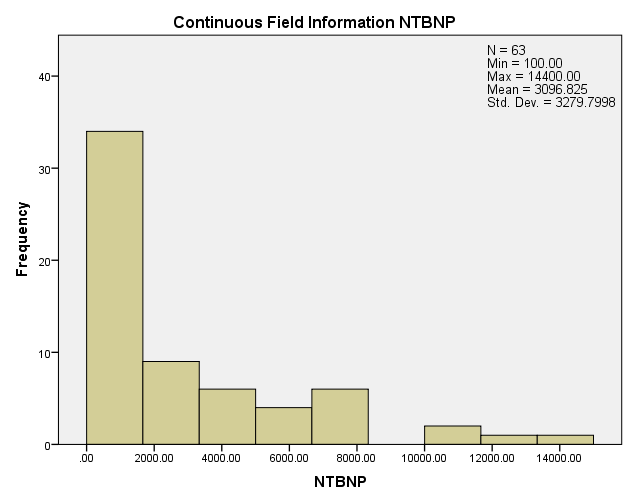
\includegraphics[scale=0.7]{./images/cont_ntprobnp.png}
    \caption{}
    \label{}
\end{figure}

\clearpage
\begin{figure}
    \centering
    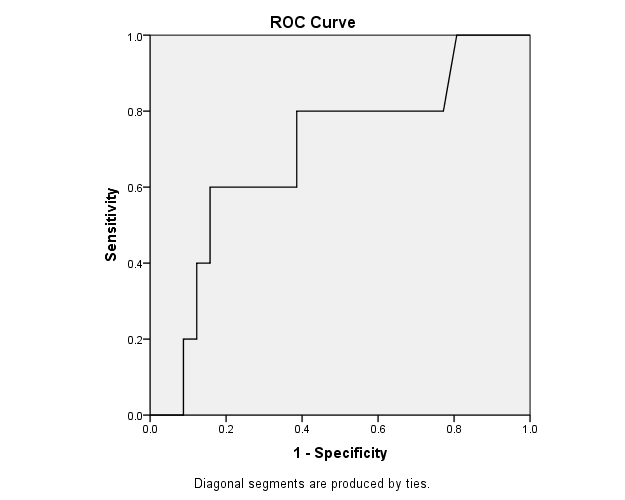
\includegraphics[scale=0.7]{./images/roc_low_co.png}
    \caption{Receiver operating characteristic curve for the ability of NT-proBNP to predict postoperative low output heart failure. area under curve = 0.69; 95\%CI = 0.44-0.93}
    \label{}
\end{figure}

\clearpage
\begin{figure}
    \centering
    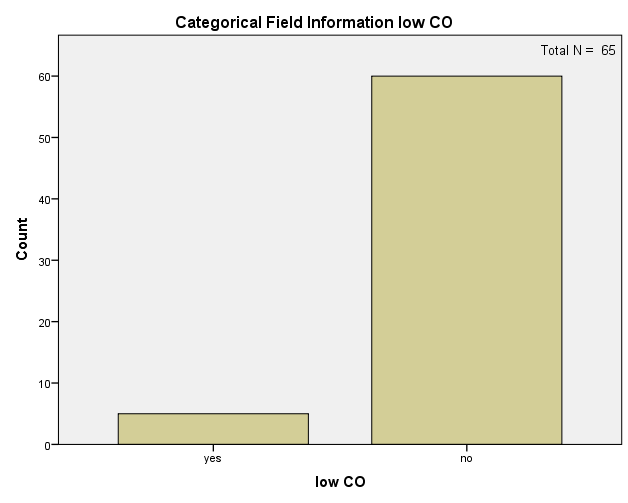
\includegraphics[scale=0.7]{./images/cat_low_co.png}
    \caption{}
    \label{}
\end{figure}

\clearpage
\begin{figure}
    \centering
    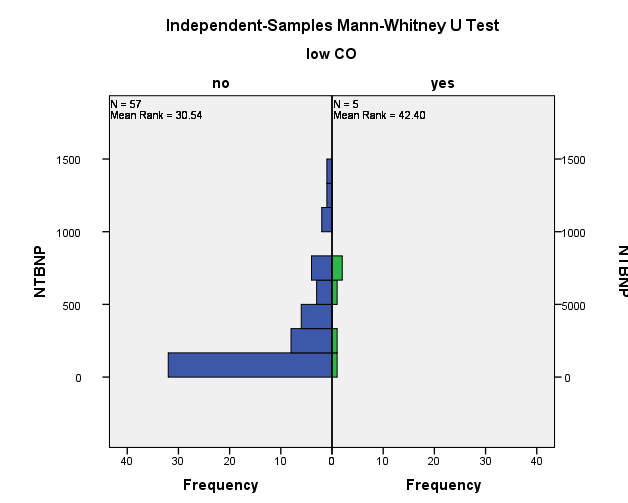
\includegraphics[scale=0.7]{./images/manwhit_low_co.png}
    \caption{}
    \label{}
\end{figure}

\clearpage
\begin{figure}
    \centering
    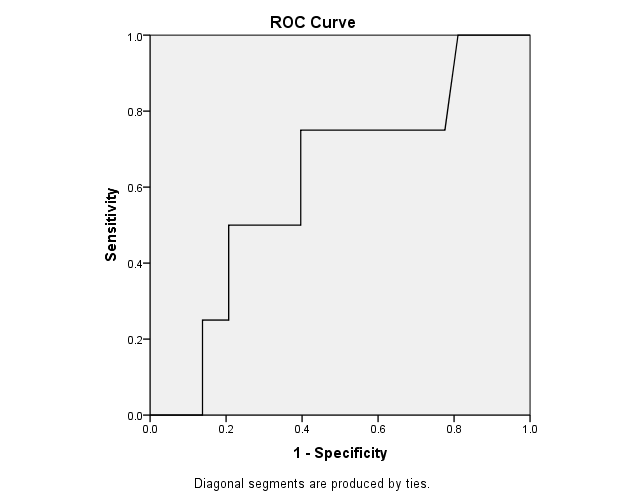
\includegraphics[scale=0.7]{./images/roc_arrhythmia.png}
    \caption{Receiver operating characteristic curve for the ability of NT-proBNP to predict postoperative arrhythmia.  area under curve = 0.61; 95\%CI = 0.35-0.88}
    \label{}
\end{figure}

\clearpage
\begin{figure}
    \centering
    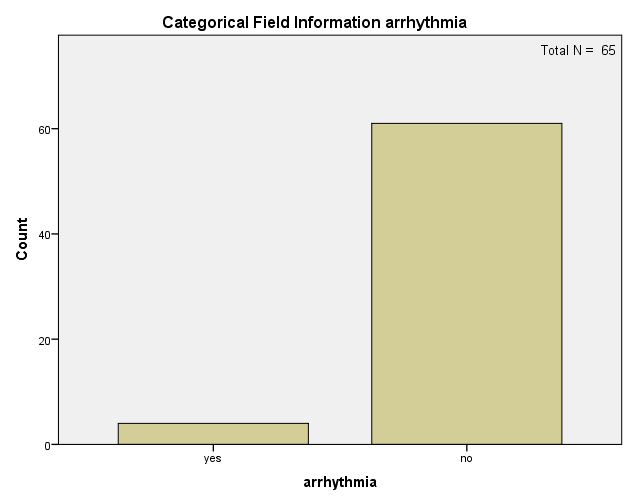
\includegraphics[scale=0.7]{./images/cat_arrhythmia.png}
    \caption{}
    \label{}
\end{figure}

\clearpage
\begin{figure}
    \centering
    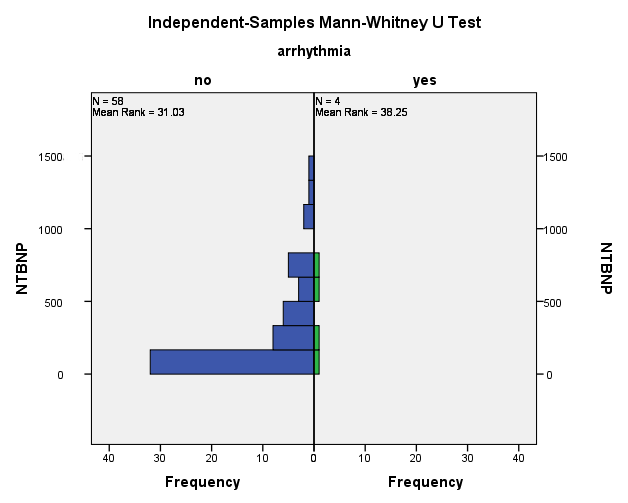
\includegraphics[scale=0.7]{./images/manwhit_arrhythmia.png}
    \caption{}
    \label{}
\end{figure}

\clearpage
\begin{figure}
    \centering
    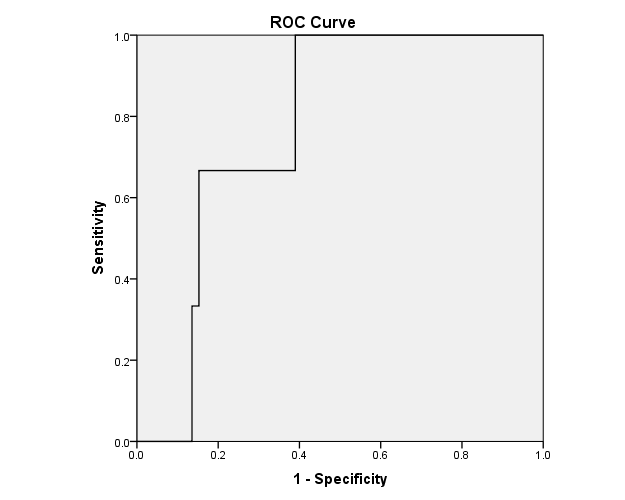
\includegraphics[scale=0.7]{./images/roc_vent.png}
    \caption{Receiver operating characteristic curve for the ability of NT-proBNP to predict prolonged postoperative mechanical ventilation.  area under curve = 0.77; 95\%CI = 0.61-0.93}
    \label{}
\end{figure}

\clearpage
\begin{figure}
    \centering
    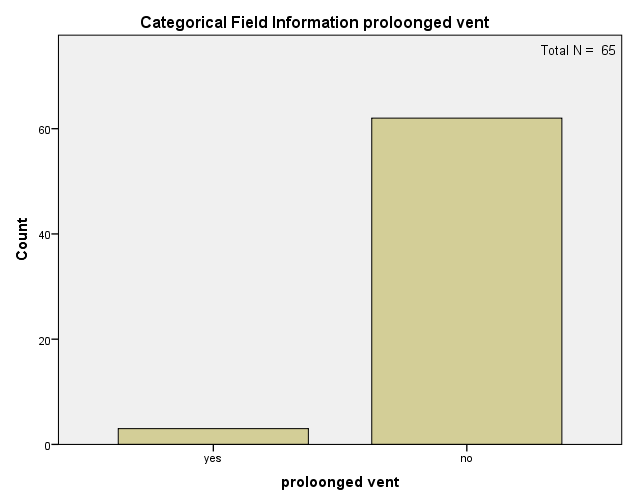
\includegraphics[scale=0.7]{./images/cat_vent.png}
    \caption{}
    \label{}
\end{figure}

\clearpage
\begin{figure}
    \centering
    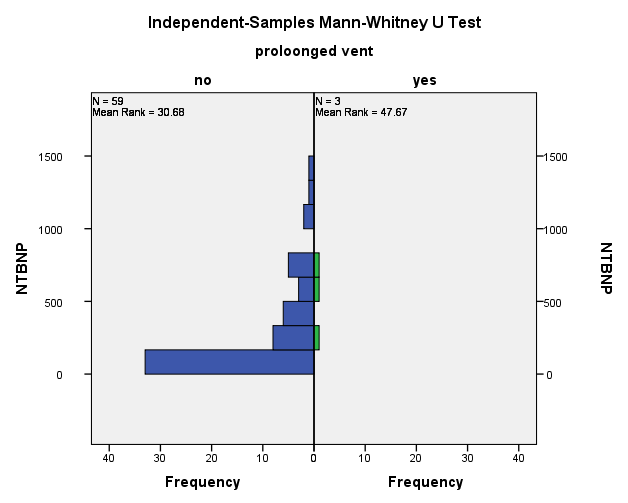
\includegraphics[scale=0.7]{./images/manwhit_vent.png}
    \caption{}
    \label{}
\end{figure}

\clearpage
\begin{figure}
    \centering
    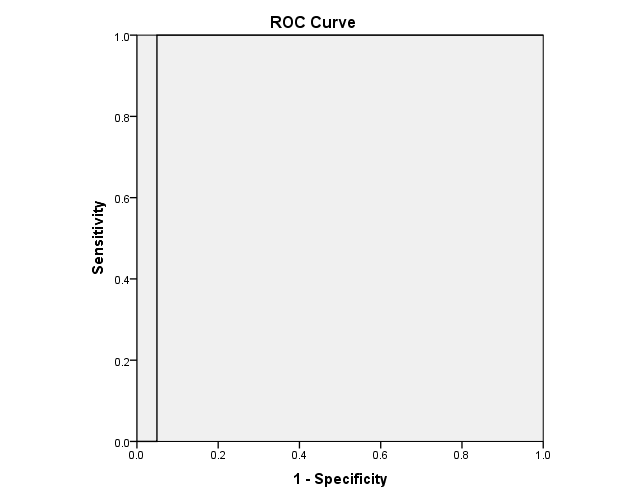
\includegraphics[scale=0.7]{./images/roc_recovery.png}
    \caption{Receiver operating characteristic curve for the ability of NT-proBNP to predict delayed postoperative neurological recovery.  area under curve = 0.95; 95\%CI = 0.89-1.0}
    \label{}
\end{figure}

\clearpage
\begin{figure}
    \centering
    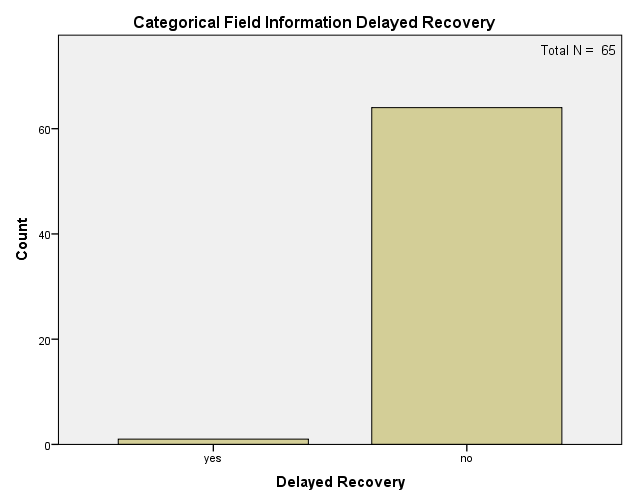
\includegraphics[scale=0.7]{./images/cat_recovery.png}
    \caption{}
    \label{}
\end{figure}

\clearpage
\begin{figure}
    \centering
    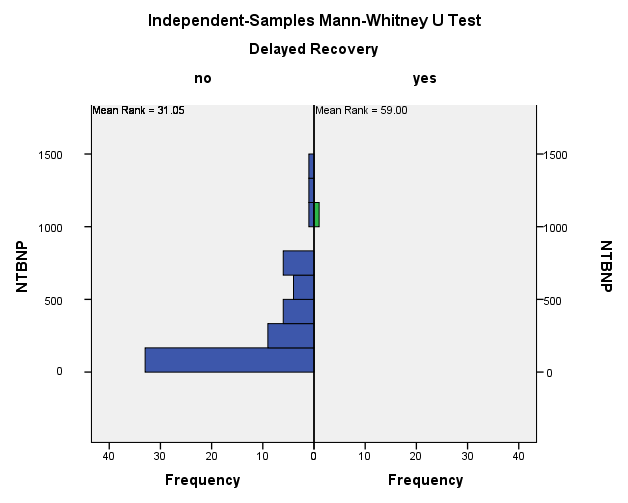
\includegraphics[scale=0.7]{./images/manwhit_recovery.png}
    \caption{}
    \label{}
\end{figure}

\clearpage
\begin{figure}
    \centering
    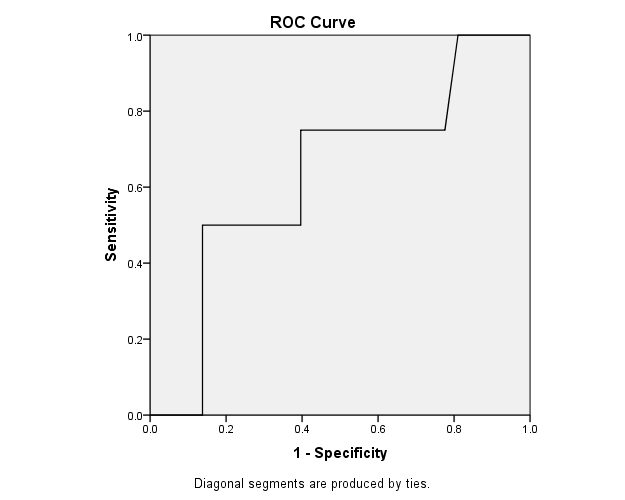
\includegraphics[scale=0.7]{./images/roc_mi.png}
    \caption{Receiver operating characteristic curve for the ability of NT-proBNP to predict perioperative myocardial infarction.  area under curve = 0.63; 95\%CI = 0.35-0.91}
    \label{}
\end{figure}

\clearpage
\begin{figure}
    \centering
    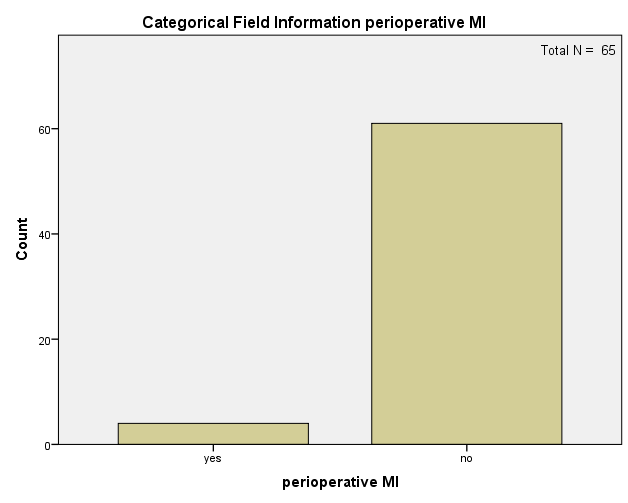
\includegraphics[scale=0.7]{./images/cat_mi.png}
    \caption{}
    \label{}
\end{figure}

\clearpage
\begin{figure}
    \centering
    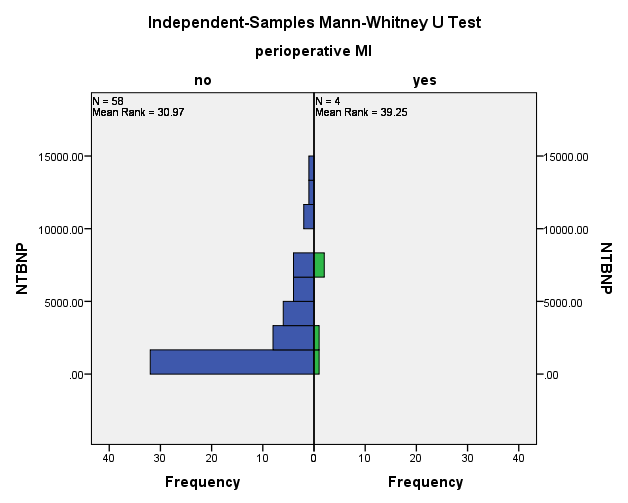
\includegraphics[scale=0.7]{./images/manwhit_mi.png}
    \caption{}
    \label{}
\end{figure}

\clearpage
\begin{figure}
    \centering
    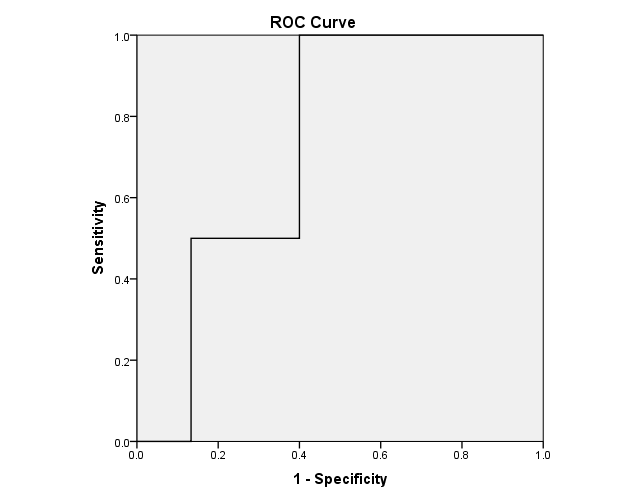
\includegraphics[scale=0.7]{./images/roc_mort.png}
    \caption{Receiver operating characteristic curve for the ability of NT-proBNP to predict in-hospital mortality.  area under curve = 0.73; 95\%CI = 0.52-0.94}
    \label{}
\end{figure}

\clearpage
\begin{figure}
    \centering
    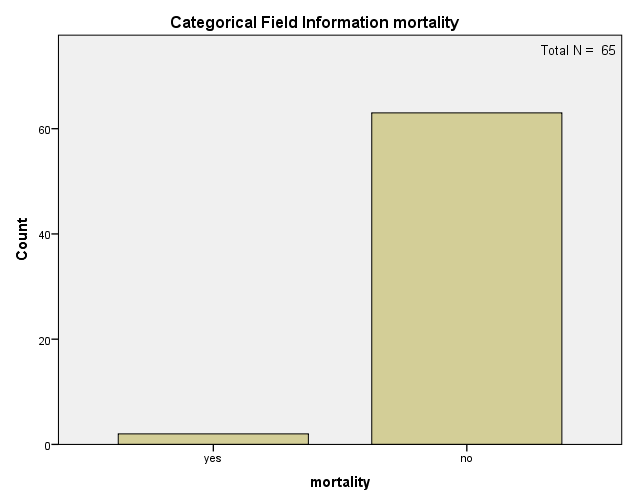
\includegraphics[scale=0.7]{./images/cat_mort.png}
    \caption{}
    \label{}
\end{figure}

\clearpage
\begin{figure}
    \centering
    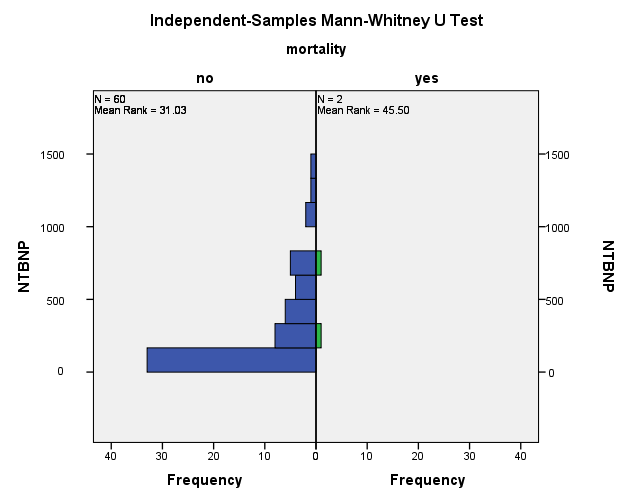
\includegraphics[scale=0.7]{./images/manwhit_mort.png}
    \caption{}
    \label{}
\end{figure}

\clearpage
\section{Discussion}


\begin{landscape}
\begin{table}
    \centering
    \caption{design of compared studies}
    \begin{tabular}{|l|c|c|c|c|c|}
        \hline
            & \cite{Eliasdottir2008} & \cite{Schachner2010} & \cite{Krzych2011} & \cite{Chen2013} & current study \\
        \hline
        year & 2008 & 2010 & 2011 & 2013 & 2017 \\
        population/cohort & elective cardiac surgery & isolated CABG & elective on-pump CABG & elective CABG & OPCAB \\
        Number & 135 & 819 & 100 & 76 & 65 \\
        peptide measured & NTproBNP & NTproBNP & NTproBNP & BNP and NTproBNP & NTproBNP \\
        sampling time &preoperative & preoperative & preoperative & preoperative and postoperative days 1 and 7 & preoperative \\
        Follow-up & 28 days & 3 yrs & 30 days &  & till discharge \\

        \hline
    \end{tabular}
    \label{meta_studies}
\end{table}
\end{landscape}




\begin{landscape}
\begin{table}
	\centering
    \begin{tabular}{|l|c|c|c|c|c|}
        \hline
            & \cite{Eliasdottir2008} & \cite{Schachner2010} & \cite{Krzych2011} & \cite{Chen2013} & current study \\
        \hline
        male & 76\% & 77\% & 76\% & 85.5\% & 86.3\% \\
        age & 67 $[56-88]$ & 67 $[27-89]$ & $65.9\pm9.1$ & $64\pm10.2$ & $57.4\pm7.3$ \\
        NYHA I &  &  & 2\% &  &  \\
        NYHA II &  &  & 81\% &  &  \\
        NYHA III  &  &  & 17\% & 5\% & - \\
        NYHA IV &  &  & - &  & - \\
        \multirow{2}{*}{EF} &  &  &  & $61\pm11.2$ & $51.1\pm8.3$ \\
                            &  & 51 $[10-84]$ & 52.5(45-60) &  & 49.5(44-57) \\
        HTN &  & 85\% & 67\% &  & 65.1\% \\
        DM &  & 24\% & 33\% &  &  \\
        (on insulin) &  & 6\% &  &  & 15.15\% \\
        GFR &  &  & 90(75.5-90) &  &  \\
        Creat. &  & 1 $[0.5-6.2]$ &  &  &  \\
        CRF (on dialysis) &  & 1\% &  &  & - \\
        PVD &  & 13\% & 12\% &  & 1.5\% \\
        carotid disease &  & 7\% & 4\% &  &  \\
        COPD &  &  & 28\% &  &  \\
        EUROSCORE (logarithmic) & 8.15 & 2.51 $[1-63]$ &  &  & $0.75\pm0.34$\footnote{EUROSCORE II} \\
        operation & & & & & \\
        on-pump CABG & 56\% &  &  & 71\% &  \\
        OPCAB & 12\% &  &  & 14.47\% &  \\
        mininally invasive CABG &  &  &  & 14.47\% &  \\
        valve repair & 12\% &  &  &  &  \\
        CABG and valve repair & 20\% &  &  &  &  \\
        urgent operation & - & 17\% &  &  & - \\
        peptide level pg/mL & & & & & \\
        BNP &  &  &  & $103.8\pm184$ &  \\
        \multirow{2}{*}{NTproBNP} & $1223\pm470$ &  $[6-65998]$ &  & $621.3\pm1050.7$ & $309.68\pm327.9$ \\
                                  & 237 (75-899) & 291(123-808) & 526(156-1150) &  & 160(80-395) \\

        \hline
    \end{tabular}
    \caption{pre-operative variables in compared studies}
    \label{meta_preoperative}
\end{table}
\end{landscape}


\begin{landscape}
\begin{table}
	\centering
    \caption{post-operative variables in compared studies}
    \begin{tabular}{|l|c|c|c|c|c|}
        \hline
            & \cite{Eliasdottir2008} & \cite{Schachner2010} & \cite{Krzych2011} & \cite{Chen2013} & current study \\
        \hline


        prolonged ventilation &  & 8 $[0-1900]$ h & 15\% &  & 4.62\% \\
        respiratory failure &  &  & 2\% &  &  \\
        atrial fibrillation &  & 23\% & 34\% &  & 6.15\% \\
        perioperative MI & 14.1\% & 1\% & 2\% &  & 6.15\% \\
        low CO &  &  & 9\% &  & 7.69\% \\
        inotropes & 33\% &  & 61\% &  &  \\
        IABP & 10\% & 4\% & 7\% &  &  \\
        stroke/delerium &  & 0.5\% & 1\% &  & 1.54\% \\
        \multirow{2}{*}{ICU stay} &  & 22 $[7-1919]$ h &  &  & $3.37\pm0.84$ days \\
                                  & 22\% &  &  &  & 23\% \\
        Hospital stay &  &  &  &  & $6.38\pm1.33$ \\
        mortality & 5.9\% & 4\% & - &  & 3\% \\

        \hline
    \end{tabular}
    \label{meta_postoperative}
\end{table}
\end{landscape}


\begin{landscape}
\begin{table}
	\centering
    \caption{correlation of peptide levels with post-operative variables in compared studies}
    \begin{tabular}{|l|c|c|c|c|}
        \hline
            & \cite{Schachner2010} & \cite{Krzych2011} & \cite{Chen2013} & current study \\
        \hline

        \hline
    \end{tabular}
    \label{meta_correlation}
\end{table}
\end{landscape}



Steady-state levels of NT-proBNP are as much as four-to six-fold higher than BNP. We used NT-proBNP instead of BNP because of its longer plasma half-life (60-120 min). The longer half-life of NT-proBNP suggests it is more independent of inter- and intra-individual variations \citep{Clerico2006}. Furthermore, molecules of BNP are unstable at room temperature and start degrading immediately after blood draw if not processed. And in their relation to clinical characteristics and prognostic performance in a large population of patients with heart failure, BNP and NT-proBNP showed subtle differences \citep{Masson2006}.

BNP and NTproBNP are simple laboratory tests with the results easily reproduced and corroborated. Several investigators demonstrated that plasma BNP and NT-proBNP concentrations are good predictors for outcome of cardiac surgery \citep{Hutfless2004}. Eliasdottir et al. showed that preoperative NT- proBNP concentration was significantly higher in patients with prolonged ICU stay, death within 28 postoperative days, required inotropic agents or IABP, and new development of postoperative renal failure and also found a good correlation between NT-proBNP and euroSCORE \citep{Eliasdottir2008}.  However, these two studies were not adjusted for the risk factors that could influence the BNP level, NT-proBNP level, morbidity, and mortality.

% describe the data in tables in detail for better clarity and to fill up space ;)
We are aware of four previous studies that tried to answer the same question of the current thesis; is preoperative natriuretic peptides of prognostic value when it comes to cardiac surgery patients.  The tables shown in this section shows the differences and similarities between those studies in design; cohort characteristics, peptide used and frequency and timing of samples, variables observed and duration, and their results.




Schachner et al. concluded in their study (N=819) that high preoperative levels , with cutoff value of 504 pg/mL; of NTproBNP predict mid-term mortality after CABG and are associated with significantly higher hospital mortality and perioperative complications.  Age, preoperative serum creatinine, peripheral vascular disease, and high NT-proBNP levels were significantly associated with hospital mortality.  Their study was more permissive than ours, including all patients undergoing isolated CABG. \citep{Schachner2010}

Krzych et al.; in a study published 2011 (N=100) found the preoperative NT-proBNP level was a predictor of postoperative prolonged mechanical ventilation, respiratory failure, AF, IABP use, inotropic support and postoperative platelet transfusions. However, good or very good diagnostic accuracy was found only in relation to mechanical ventilation, respiratory insufficiency, IABP use, and milrinone use, with cutoff value of 1032-1443 pg/mL. No deaths were observed in their study. \citep{Krzych2011}  Like our study, they included only patients scheduled for elective surgery with EF $> 30\%$ and without renal failure.

In a study, Chen et al. (N=76) demonstrated that postoperative Day 1 BNP and NT-proBNP concentrations were significantly higher in patients with prolonged ICU stay and hospitalization. However, the correlation became insignificant after adjusting for age, sex,  renal function, and LVEF \citep{Chen2013}. Moreover, they stated that high postoperative Day 1 BNP and NT-proBNP concentrations did not show significant correlation with prognosis after other risk factor adjustments.  In their study preoperative BNP and NTproBNP were not significantly associated with outcomes.


\section{Conclusion}

This study suggests that preoperative NTproBNP levels don't correlate with postoperative outcomes for patients who have good ejection fraction, are not in heart failure, and are undergoing elective isolated CABG surgery. This is supported by similar, albeit small-sample studies.  However, the small sample size may result in statistical bias. Therefore, a large-scale study and long-term follow-up should be performed in the future.


\section{Summary}

\newpage

\bibliography{thesis}

\end{document}
